\documentclass[../main.tex]{subfiles}

\begin{document}
	\section{Verschiedenes}
	\todo[inline]{Festlegen von Coding-Standards}
	
	\subsection{Ausbaumöglichkeiten}
	\par Wenn das Projekt gemäss Kapitel \nameref{section:Akzeptanzkriterien} umgesetzt wurde, bestehen diverse Möglichkeiten, den Umfang des Projekts zu erweitern. Neben zusätzlichen Kombinationen von Plättchentyp, -art und -verhalten, stehen unter anderem folgende Punkte als Ausbaumöglichkeit zur Verfügung:
	\begin{itemize}
		\item Möglichkeit, Plättchenstapel neu zu mischen
		\item Möglichkeit, Plättchen zu kombinieren
		\item Spielfelder mit bereits bestehenden Besonderheiten
		\item Online \gls{highscore} Rangliste
		\item Zusätzliche Spielmodi
		\begin{itemize}
			\item Vorgefertigte, begrenzte Spielfelder
			\item Zeitliche Begrenzungen
		\end{itemize}
	\end{itemize}
	\subsection{Coding-Standard}
	\par Das Team wird sich am bereits bekannten Coding-Standard der ZHAW orientieren und ihn, falls angebracht, in bestimmten Gebieten anpassen. Diese Anpassungen werden sich auf bestehende \glspl{bestpractice} für \gls{csharp} und \gls{unity} stützen.
	\subsection{Artefakte}
	
	\begin{figure}[H]
		\centering
		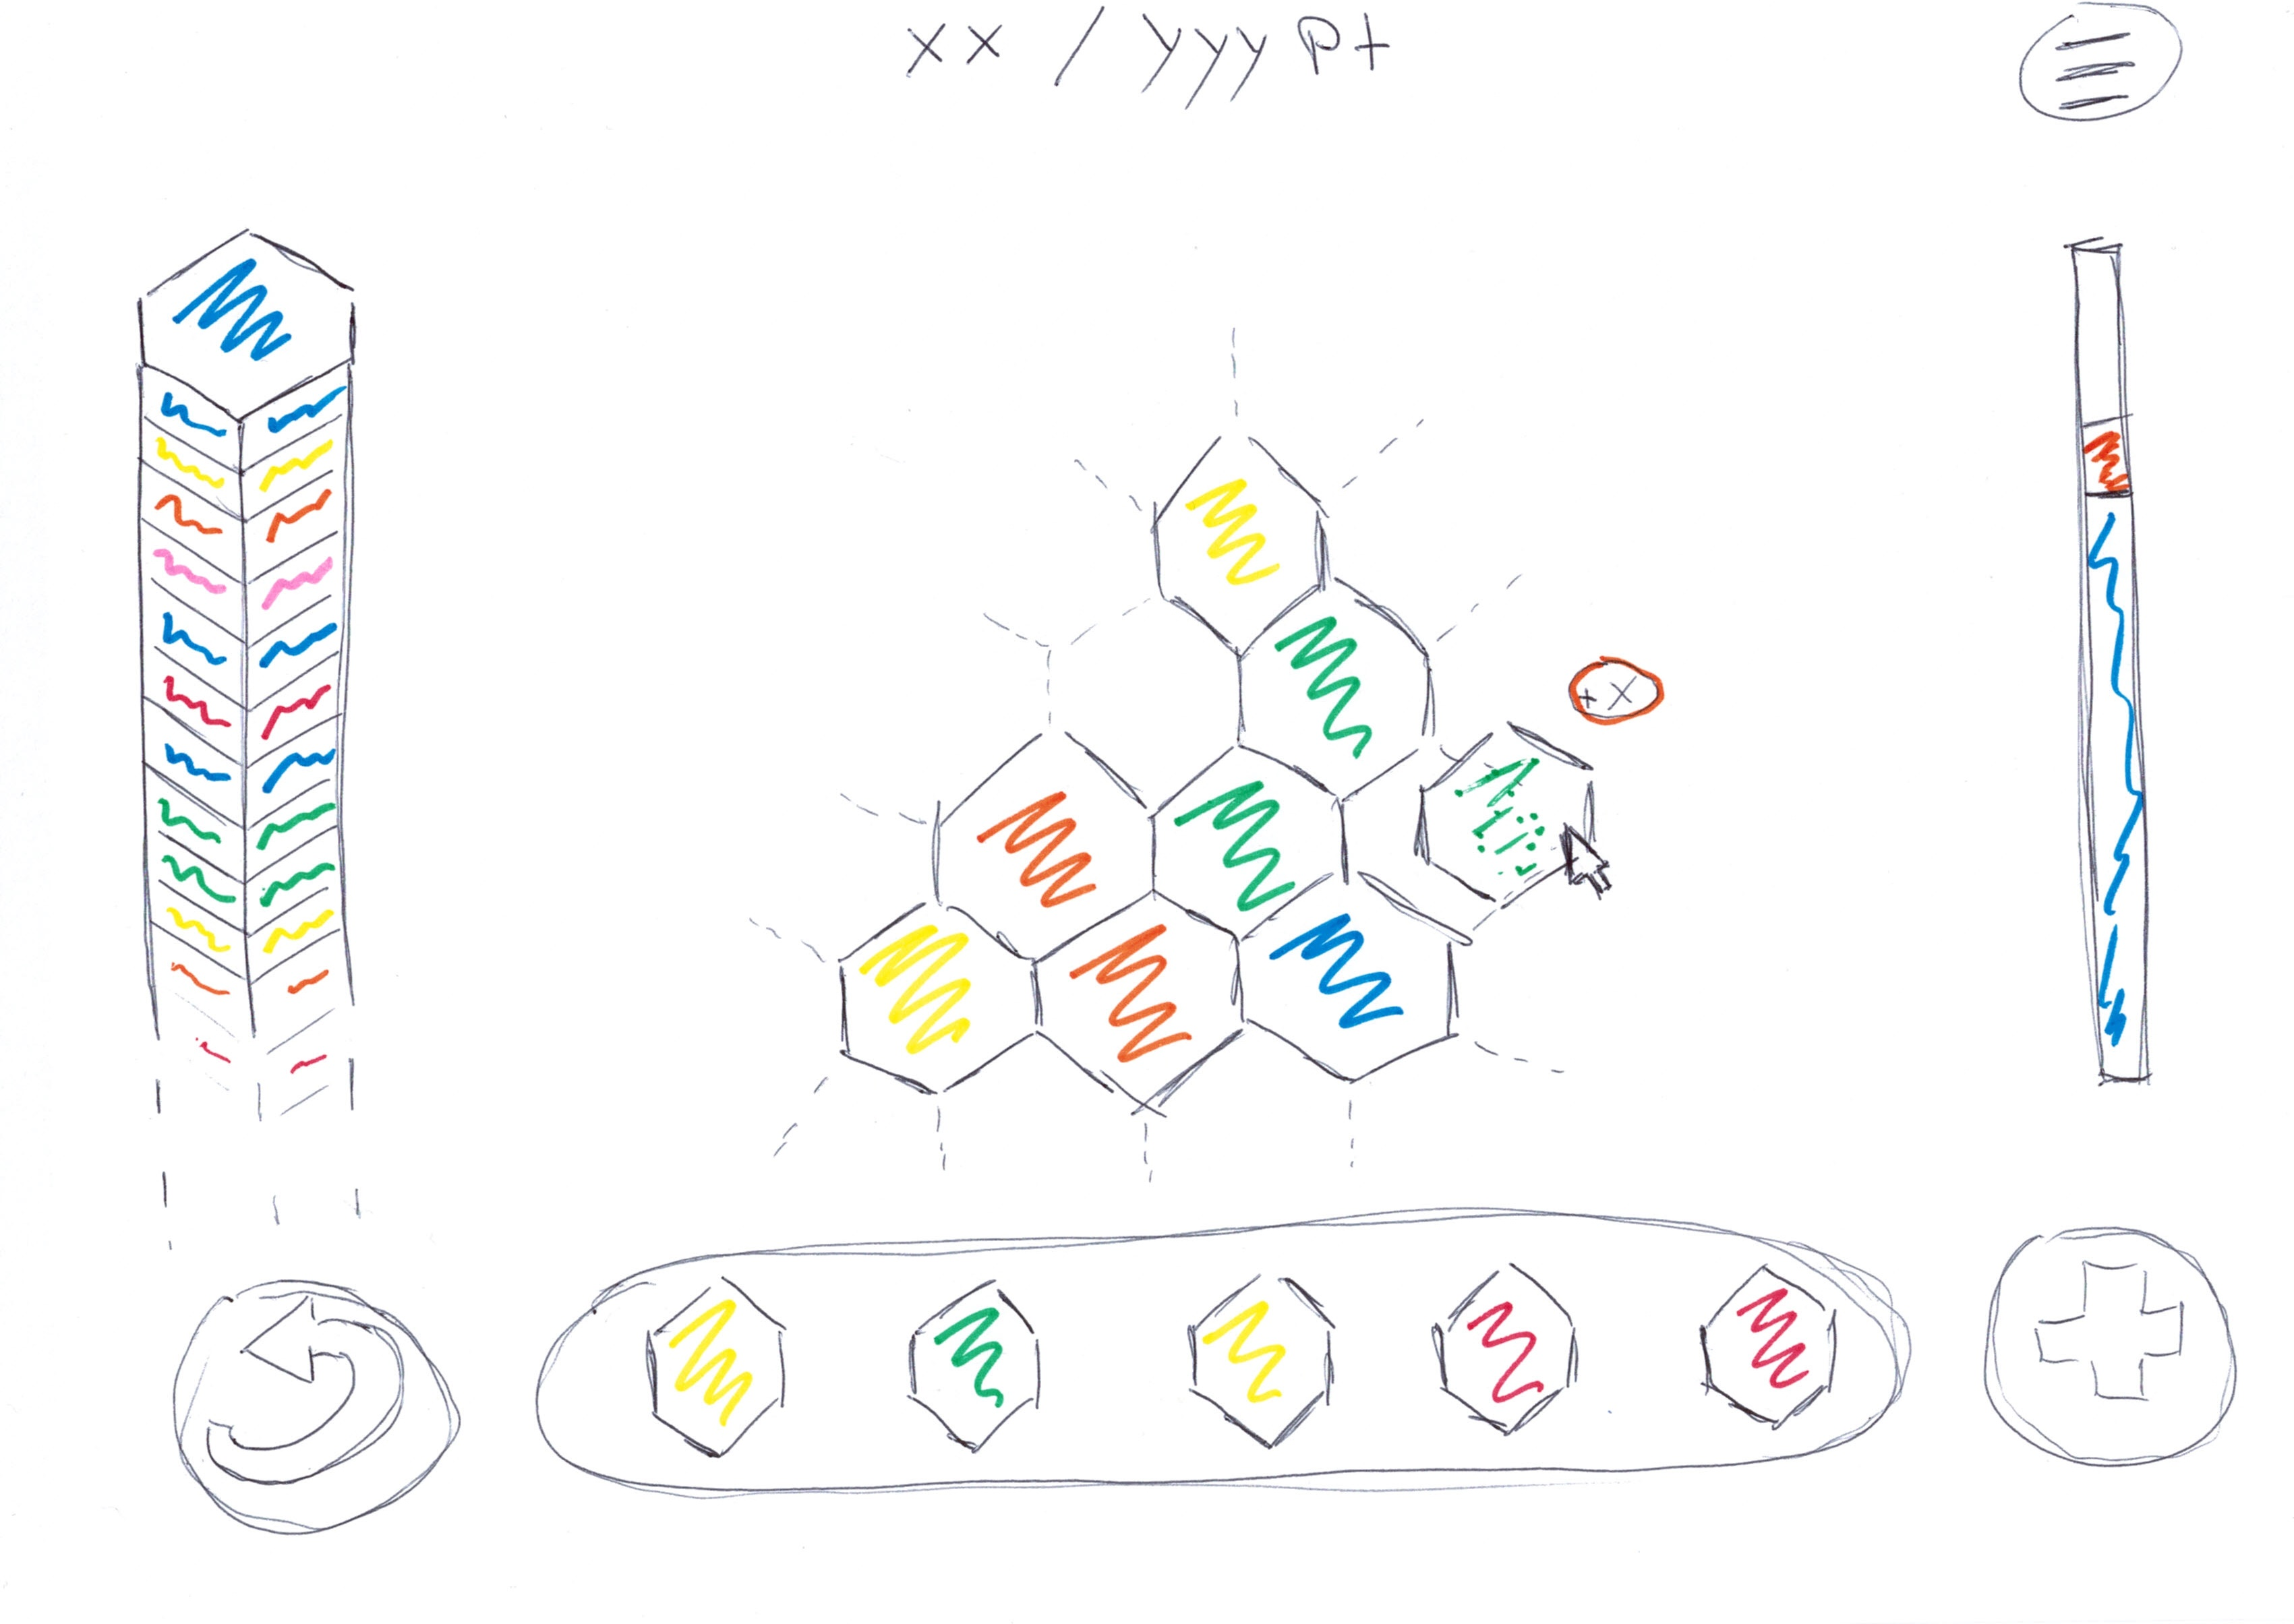
\includegraphics[width=0.5\linewidth]{Hexxle_Concept_UI.jpg}
		\caption{}
	\end{figure}

	\begin{figure}[H]
		\centering
		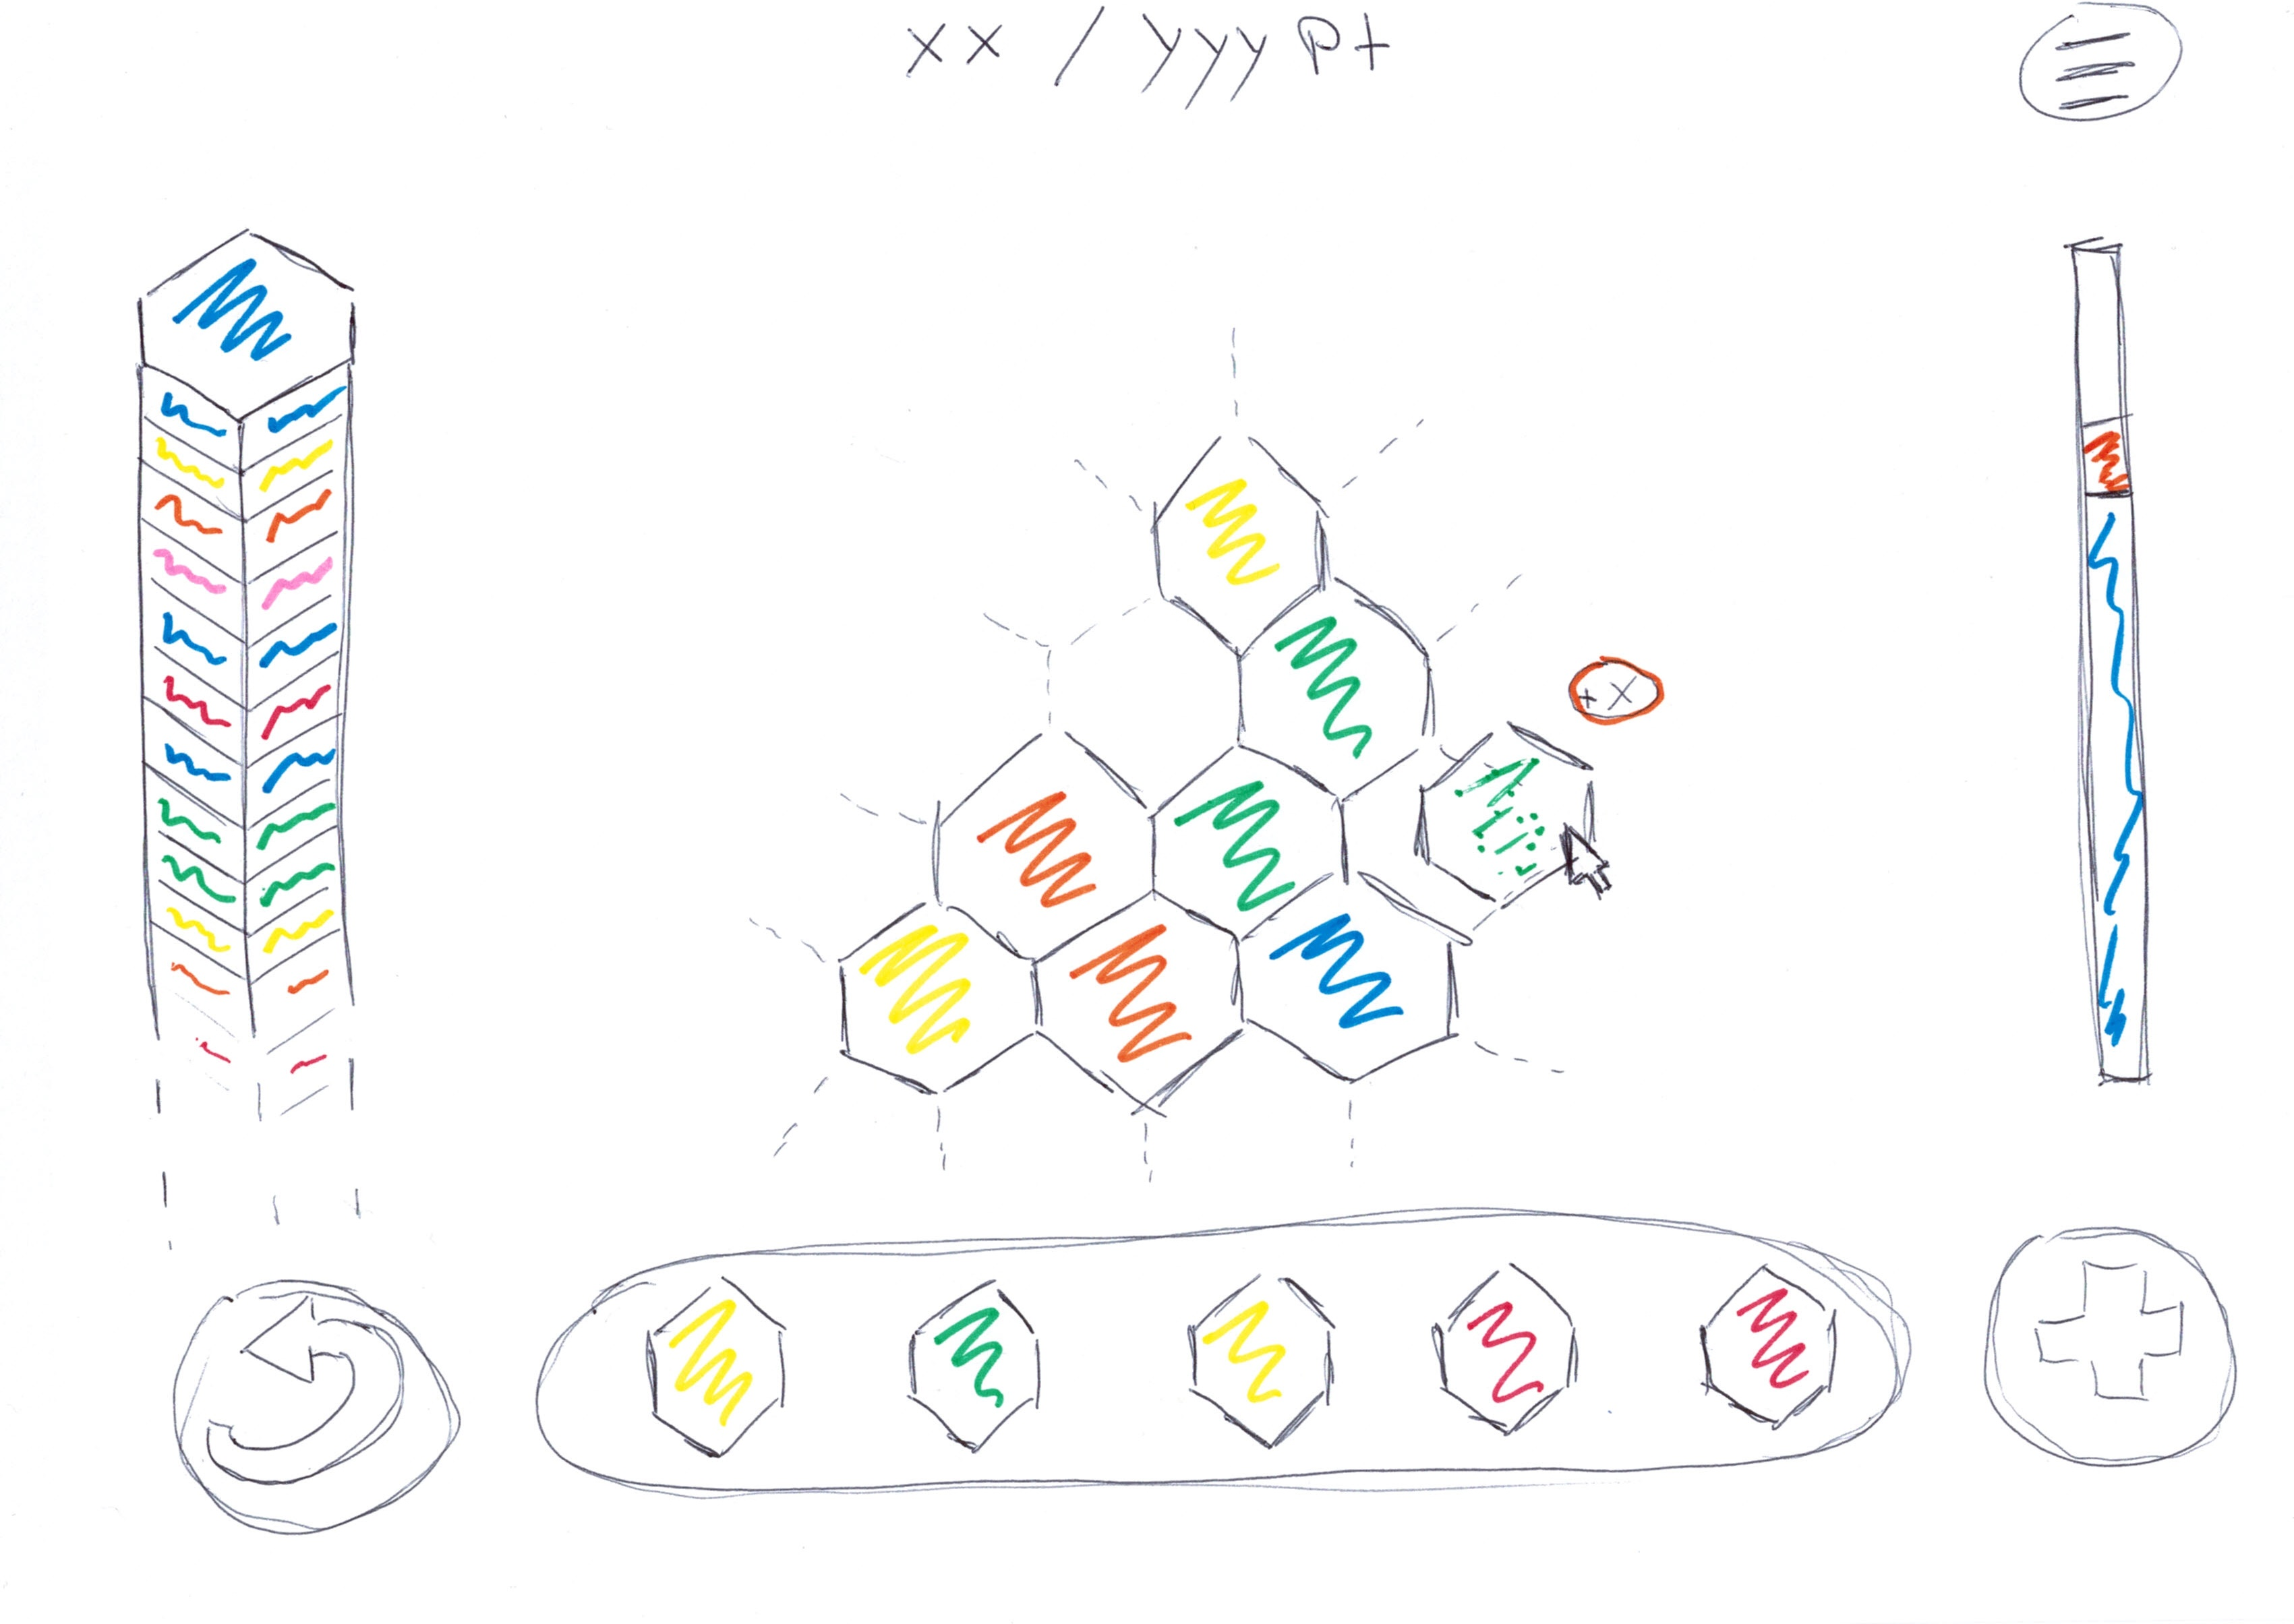
\includegraphics[width=0.5\linewidth]{Hexxle_Concept_UI.jpg}
		\caption{}
	\end{figure}

	\begin{figure}[H]
		\centering
		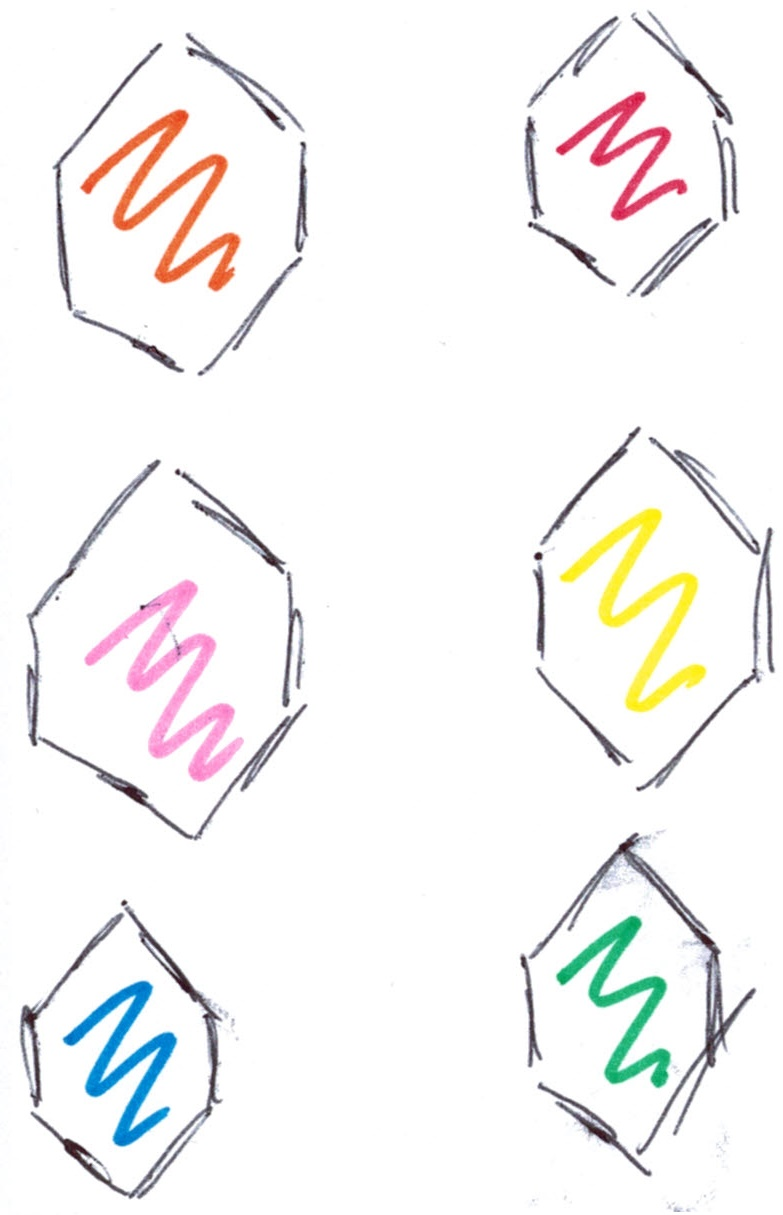
\includegraphics[width=0.5\linewidth]{Hexxle_Concept_PlaettchenTyp.jpg}
		\caption{}
	\end{figure}

	\begin{figure}[H]
		\centering
		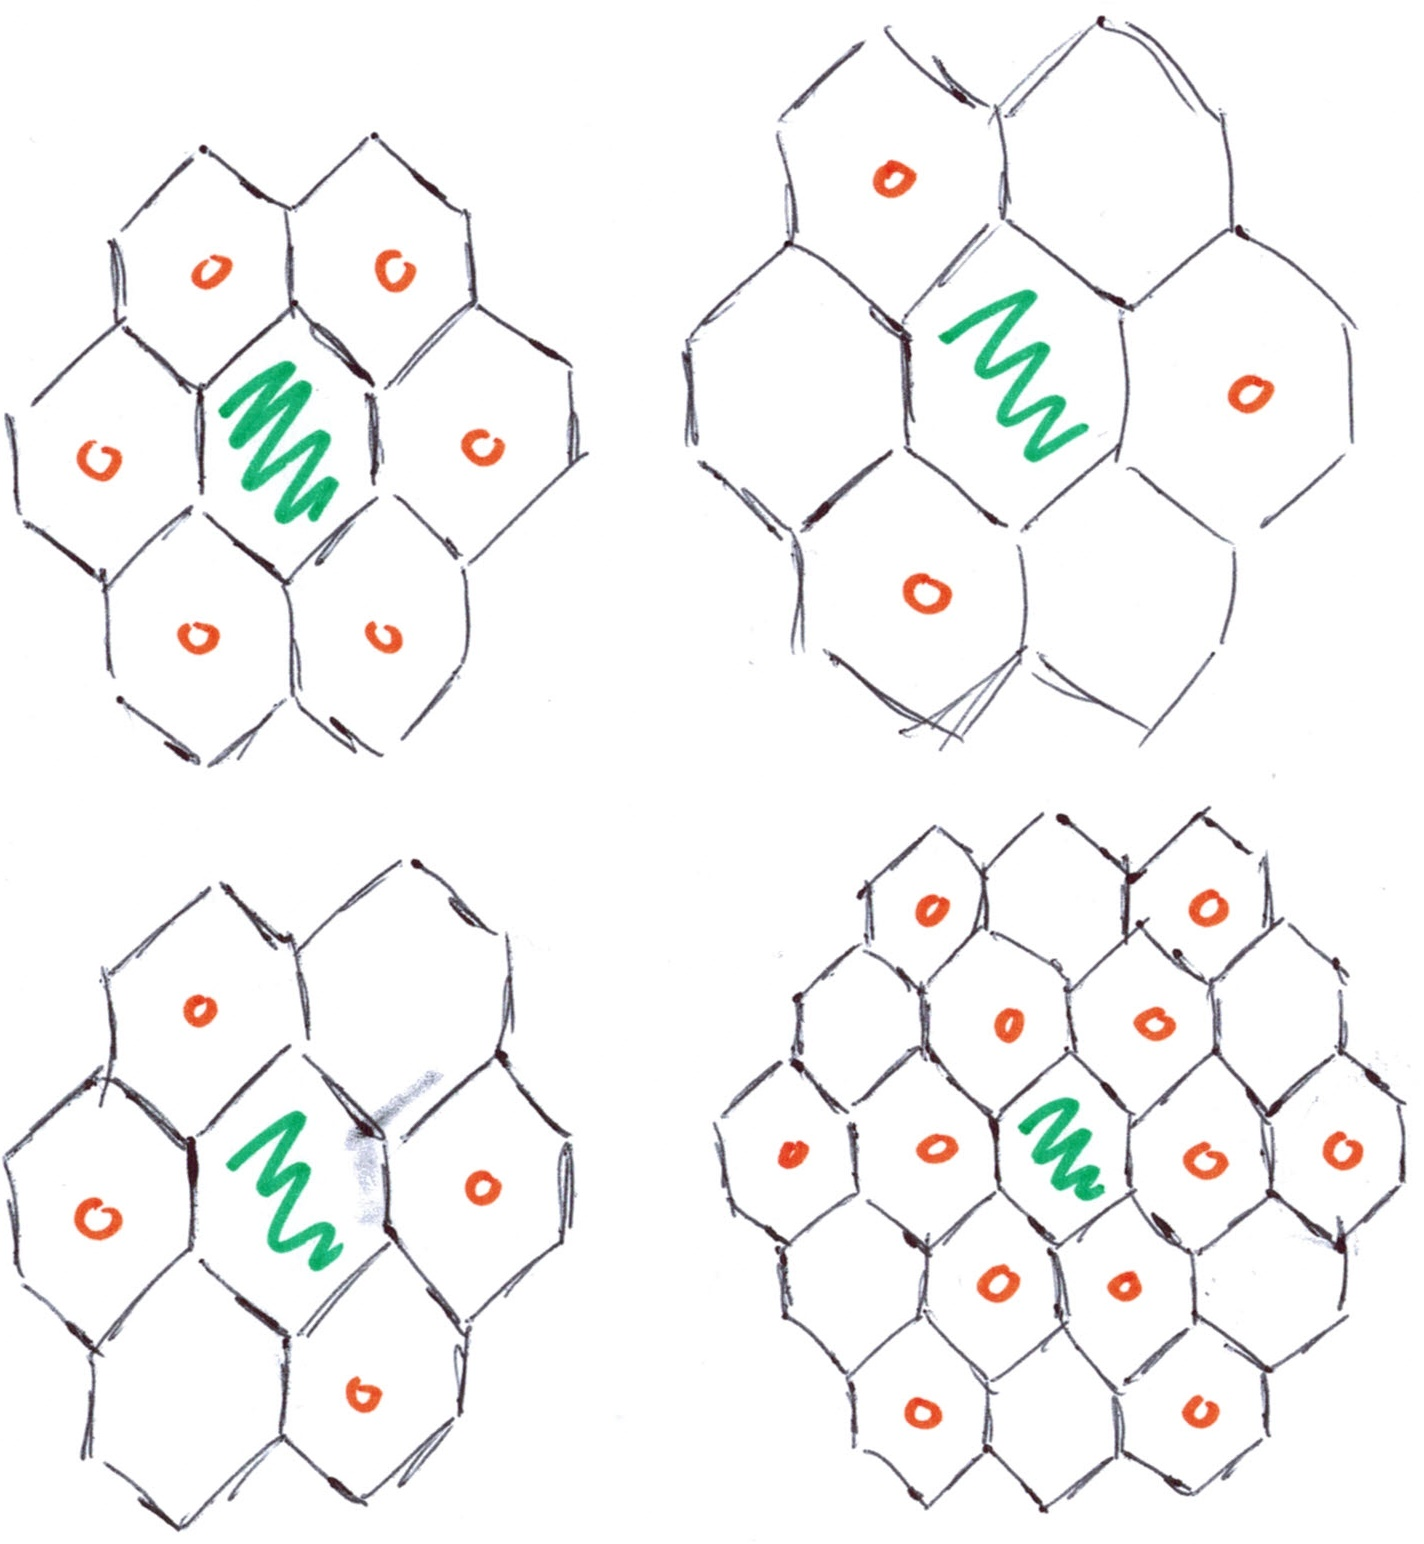
\includegraphics[width=0.5\linewidth]{Hexxle_Concept_PlaettchenArt.jpg}
		\caption{}
	\end{figure}

	\begin{figure}[H]
		\centering
		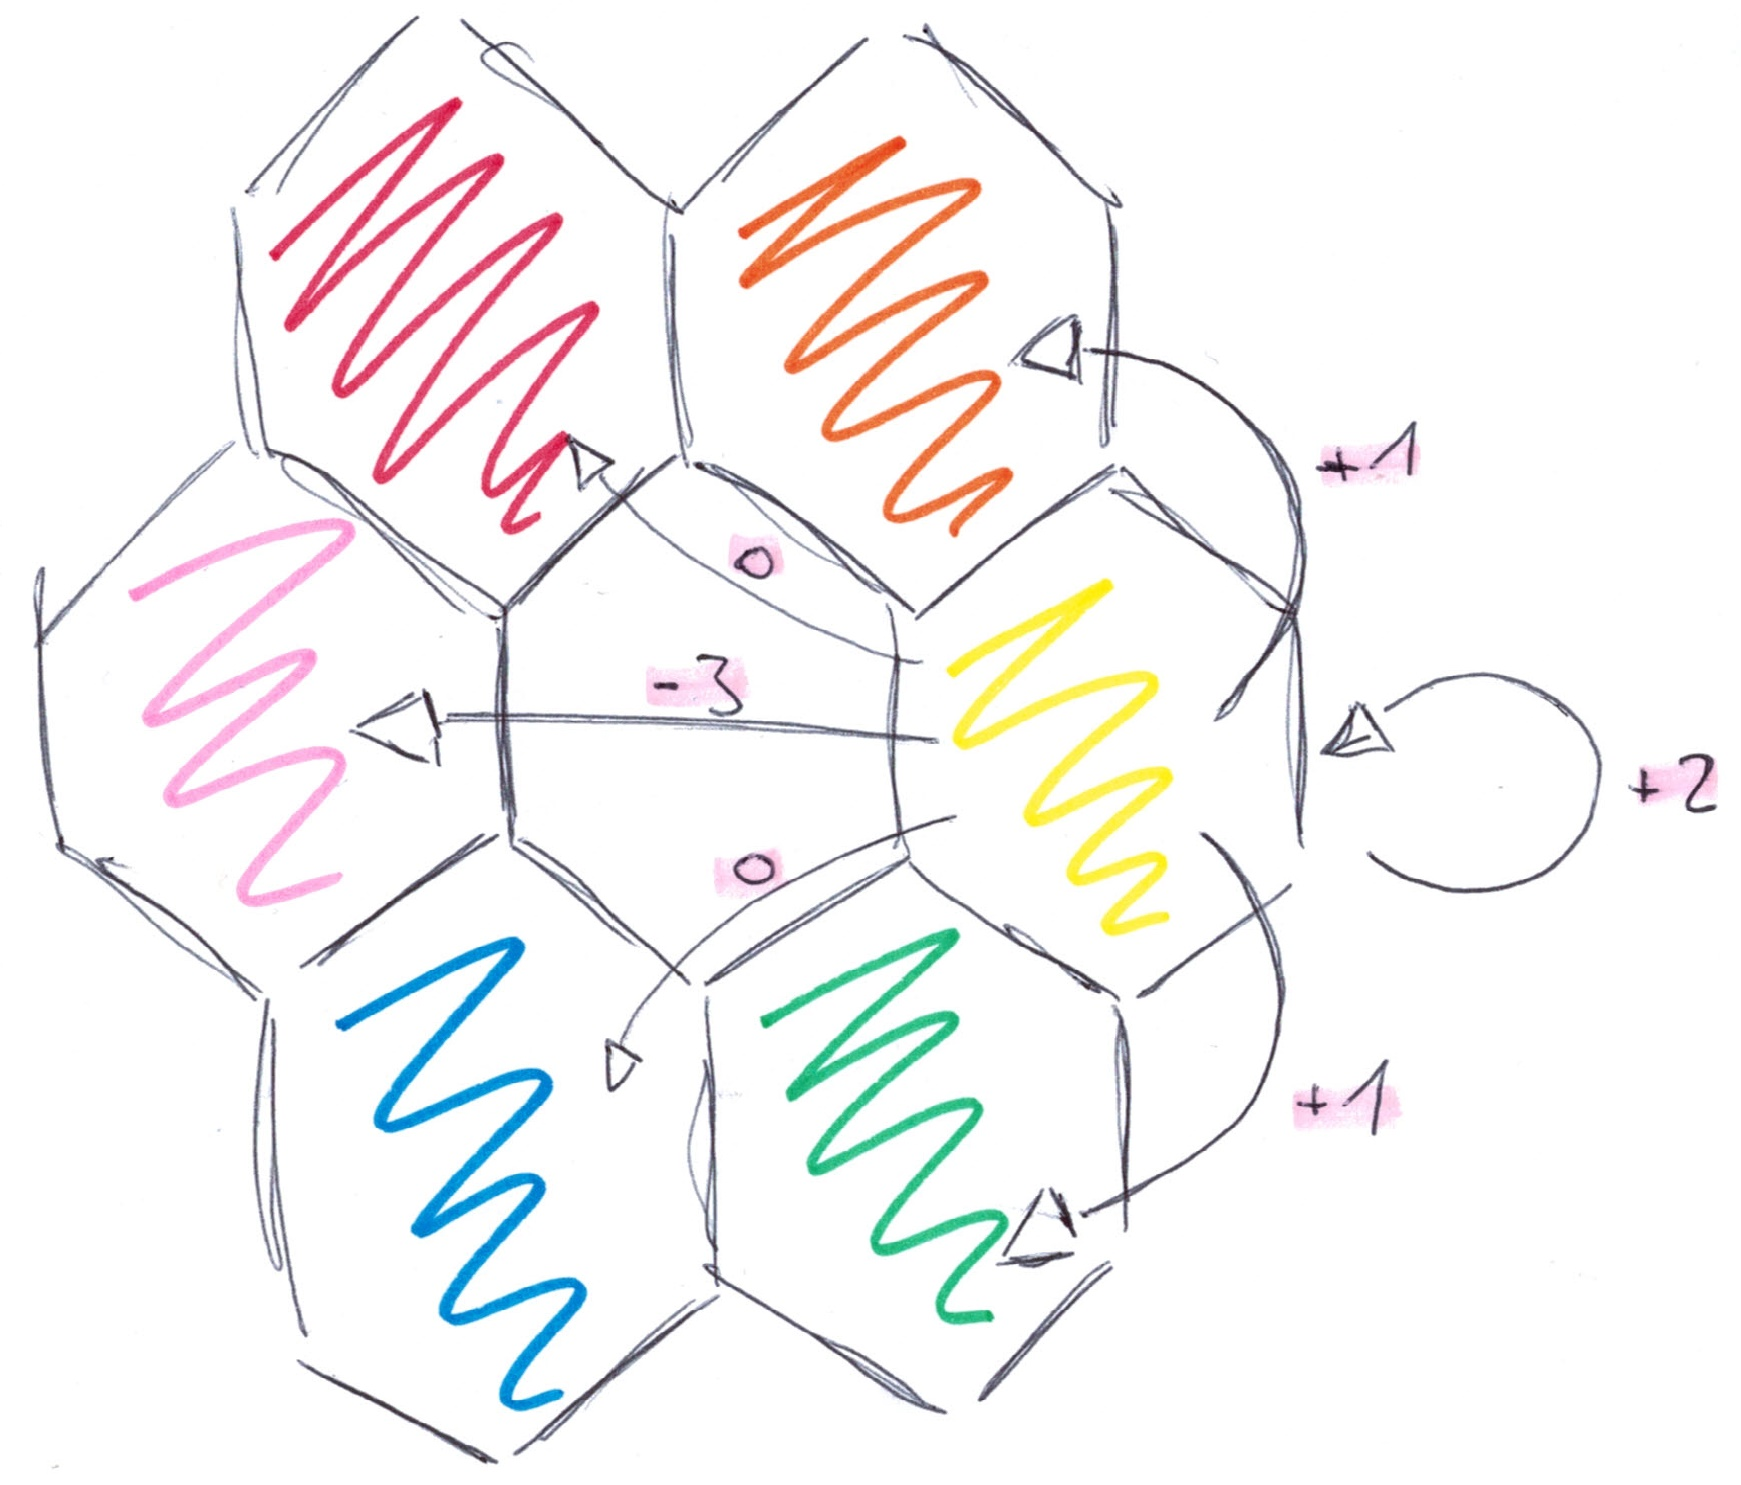
\includegraphics[width=0.5\linewidth]{Hexxle_Concept_Adjacency.jpg}
		\caption{}
	\end{figure}

	\begin{figure}[H]
		\centering
		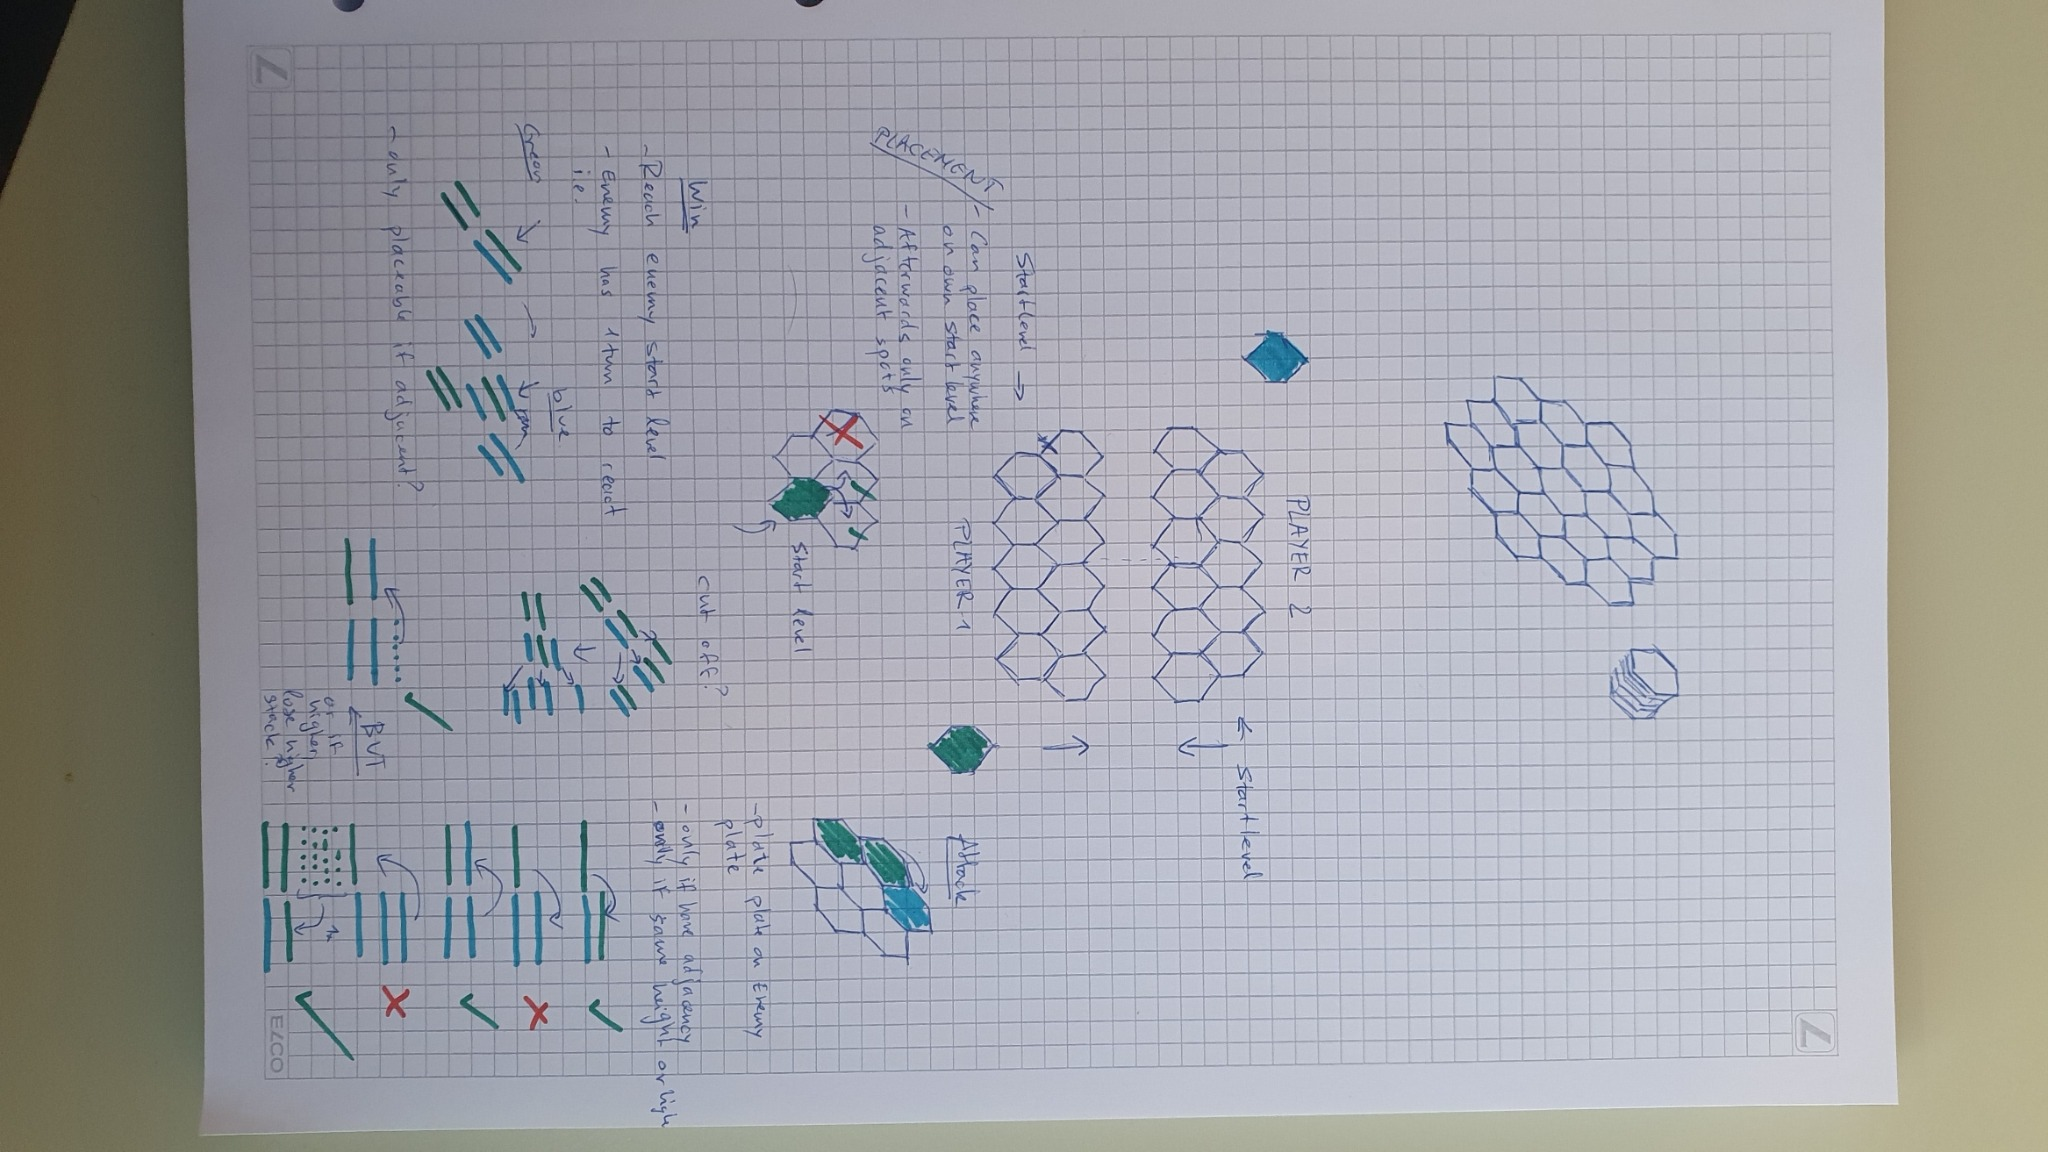
\includegraphics[width=0.5\linewidth]{RicardoBrainstorm.jpeg}
		\caption{}
	\end{figure}
\end{document}